\documentclass[compress]{beamer}
\usepackage{irbookslide}
\usepackage{irilmenau2}
\usepackage{tikz}
\usepackage{url}
\usepackage{ifxetex}
%\RequireXeTeX
\usepackage{fontspec} % zahteva paket euenc
\usepackage{xunicode}
\usepackage{xltxtra}
\usepackage{polyglossia}
\usepackage{minted}
\usepackage[noend]{algorithmic}
\renewcommand{\algorithmicrequire}{\textbf{Input:}}
\renewcommand{\algorithmicensure}{\textbf{Output:}}
\renewcommand{\algorithmiccomment}[1]{\hfill \{\myred{#1}\}}
\usepackage{xcolor,colortbl}
\usepackage{textcomp}
\usepackage{unicode-math}
%\usepackage{hyphenat}
%\setdefaultlanguage[script=Latin]{serbian}

\title{Obrada teksta}
\author{\textcopyright \ \ Goodrich, Tamassia, Goldwasser}
\institute{Katedra za informatiku, Fakultet tehničkih nauka, Univerzitet u
Novom Sadu}
\date{2014.}
\subject{Predavanja sa ASP}

\begin{document}

\frame{\titlepage}

\section[Stringovi]{Stringovi}

\begin{frame}[fragile]
  \frametitle{String}
  \begin{itemize}
    \item \myred{string} je niz karaktera
    \item primeri stringova:
    \begin{itemize}
      \item Python program
      \item HTML dokument
      \item DNK sekvenca
      \item digitalna slika
    \end{itemize}
    \item \myred{alfabet} $\Sigma$ je skup mogućih karaktera za familiju stringova
    \item primeri alfabeta:
    \begin{itemize}
      \item ASCII
      \item Unicode
      \item \{0, 1\}
      \item \{A, C, G, T\}
    \end{itemize}
  \end{itemize}
\end{frame}

\begin{frame}[fragile]
  \frametitle{String}
  \begin{itemize}
    \item neka je $P$ string dužine $m$
    \begin{itemize}
      \item \myred{podstring} $P[i..j]$ od $P$ je podsekvenca od $P$ koja sadrži
      karaktere sa rangom između $i$ i $j$
      \item \myred{prefiks} od $P$ je podstring tipa $P[0..i]$
      \item \myred{sufiks} od $P$ je podstring tipa $P[i..m-1]$
    \end{itemize}
    \item za date stringove $T$ (tekst) i $P$ (šablon, \textit{pattern})
    \textit{pattern matching} problem je pronalaženje podstringa
    od $T$ koji je jednak $P$
    \item primene:
    \begin{itemize}
      \item editori teksta
      \item mašine za pretragu (\textit{search engines})
      \item bioinformatika
    \end{itemize}
  \end{itemize}
\end{frame}

\begin{frame}[fragile]
  \frametitle{Nalaženje podstringa grubom silom}
  \begin{itemize}
    \item nalaženje \myred{grubom silom} (\textit{brute force}) poredi šablon
    $P$ sa tekstom $T$ za svaki mogući položaj $P$ u odnosu na $T$ sve dok se
    \begin{itemize}
      \item ne pronađe poklapanje
      \item ne testiraju sve pozicije
      \item \myred{sufiks} od $P$ je podstring tipa $P[i..m-1]$
    \end{itemize}
    \item gruba sila radi u $O(nm)$ vremenu
    \item primer najgoreg slučaja:
    \begin{itemize}
      \item $T = aaa \ldots ah$
      \item $P = aaah$
      \item može da se pojavi u slikama i DNK sekvencama
      \item retko u tekstovima
    \end{itemize}
  \end{itemize}
\end{frame}

\begin{frame}[fragile,shrink]
  \frametitle{Nalaženje podstringa grubom silom}
  \myred{BruteForceMatch}($T, P$)
  \begin{algorithmic}
    \REQUIRE tekst $T$ dužine $n$ i šablon $P$ dužine $m$
    \ENSURE indeks početka podstringa u $T$ jednakog $P$ ili -1 ako nije pronađen
    \FOR{$i \leftarrow 0$ \TO $n-m$}
      \STATE $j \leftarrow 0$  \COMMENT{testiramo položaj i}
      \WHILE{$j<m \land T[i+j]=P[j]$}
        \STATE $j \leftarrow j+1$
        \IF{$j=m$}
          \RETURN $i$ \COMMENT{poklapanje na $i$}
        \ELSE
          \STATE break
        \ENDIF
      \ENDWHILE
    \ENDFOR
    \RETURN -1 \COMMENT{nije pronađen}
  \end{algorithmic}    
\end{frame}

\begin{frame}[fragile,shrink=18]
  \frametitle{Gruba sila u Pythonu}
\begin{minted}[linenos=false]{python}
def find_brute_force(T, P):
  """Return the lowest index of T at which
     substring P begins (or else -1)."""
  n, m = len(T), len(P)  # introduce convenient notations
  for i in range(n-m+1): # try every potential starting index within T
    k = 0                # an index into pattern P
    while k < m and T[i + k] == P[k]: # kth character of P matches
      k += 1
    if k == m:           # if we reached the end of pattern,
      return i           # substring T[i:i+m] matches P
  return -1              # failed to find a match starting with any i
\end{minted}
\end{frame}

\begin{frame}[fragile]
  \frametitle{Boyer-Moore}
  \begin{itemize}
    \item \myred{Boyer-Moore} algoritam se zasniva na dve heuristike
    \begin{itemize}
      \item \myred{ogledalo}: traži $P$ u $T$ unazad
      \item \myred{skok}: ako se razlika otkrije u $T[i]=c$
      \begin{itemize}
        \item ako $P$ sadrži $c$, pomeri $P$ tako da se $T[i]$ poklopi sa
        poslednjom pojavom $c$ u $P$
        \item inače pomeri $P$ tako da se poklope $P[0]$ i $T[i+1]$
      \end{itemize}
    \end{itemize}
  \end{itemize}
  \begin{center}
    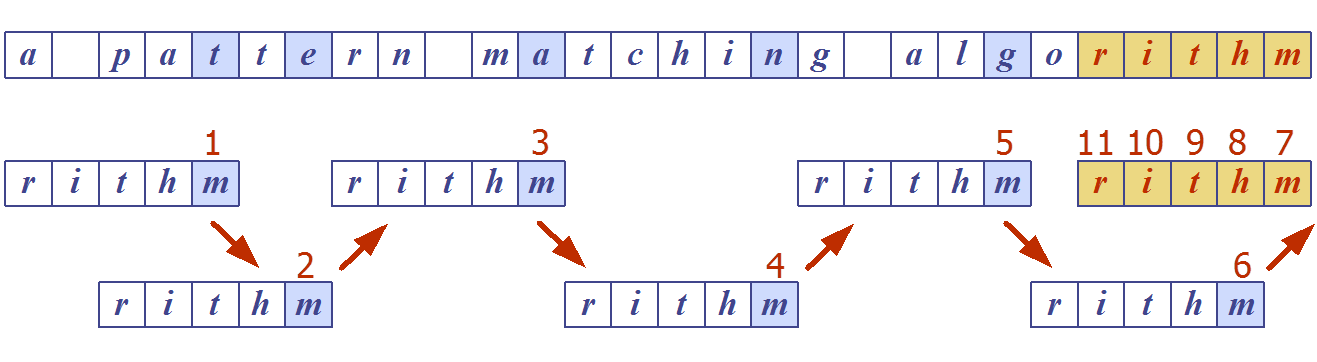
\includegraphics[width=11cm]{asp-13-pic01.png}
  \end{center}
\end{frame}

\begin{frame}[fragile]
  \frametitle{BM: funkcija poslednjeg pojavljivanja}
  \begin{itemize}
    \item Boyer-Moore algoritam formira \myred{last occurence} funkciju $L$ koja
    mapira $\Sigma$ na cele brojeve gde je $L(c)$ definisano kao
    \begin{itemize}
      \item najveći indeks $i$ takav da $P[i]=c$
      \item -1 ako takvog indeksa nema
    \end{itemize}
    \item primer: $\Sigma = \{a,b,c,d\} \quad P = abacab$
  \end{itemize}
  \begin{center}
    \begin{tabular}{c||c|c|c|c}
    $c$ & $a$ & $b$ & $c$ & $d$ \\ \hline
    $L(c)$ & $4$ & $5$ & $3$ & $-1$ \\
    \end{tabular}
  \end{center}
  \begin{itemize}
    \item može se predstaviti kao niz indeksiran numeričkim kodovima karaktera
    \item može se izračunati za $O(m+s)$ vreme gde je $m$ dužina $P$ a $s$ je veličina $\Sigma$
  \end{itemize}
\end{frame}

\begin{frame}[fragile,shrink]
  \frametitle{Boyer-Moore algoritam}
  \myred{BoyerMooreMatch}($T, P, \Sigma$)
  \begin{algorithmic}
    \STATE $L \leftarrow$ lastOccurence($P,\Sigma$)
    \STATE $i \leftarrow m-1$
    \STATE $j \leftarrow m-1$
    \REPEAT
      \IF{$T[i]=P[j]$}
        \IF{$j=0$}
          \RETURN $i$ \COMMENT{poklapanje na i}
        \ELSE
          \STATE $i \leftarrow i-1$
          \STATE $j \leftarrow j-1$
        \ENDIF
      \ELSE
        \STATE $l \leftarrow L[T[i]]$ \COMMENT{skok}
        \STATE $i \leftarrow i + m - \min(j, 1+l)$
        \STATE $j \leftarrow m-1$
      \ENDIF
    \UNTIL{$i>n-1$}
    \RETURN $-1$ \COMMENT{nije pronađen}
  \end{algorithmic}    
\end{frame}

\begin{frame}[fragile]
  \frametitle{Boyer-Moore}
  \begin{center}
    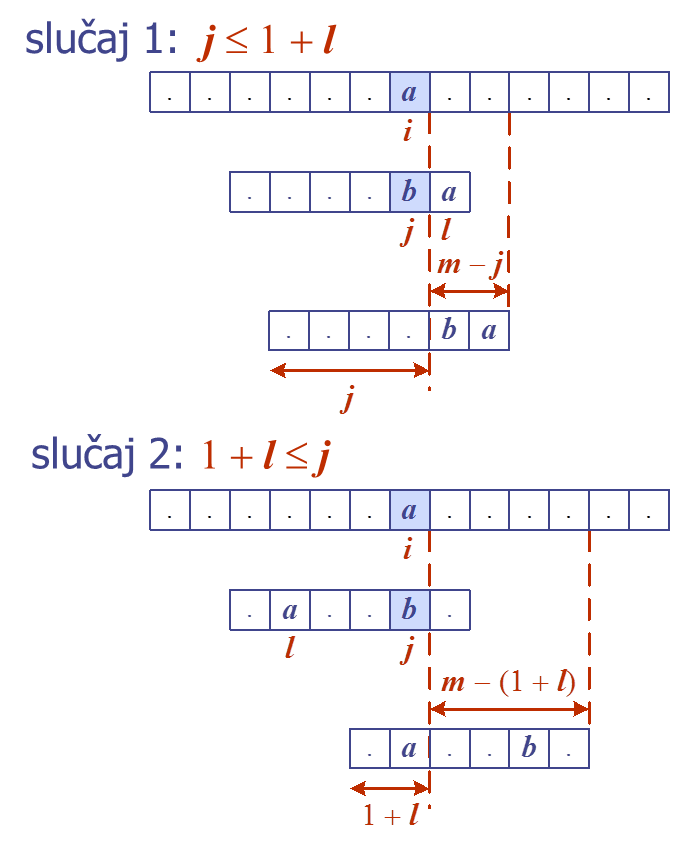
\includegraphics[width=6cm]{asp-13-pic02.png}
  \end{center}
\end{frame}

\begin{frame}[fragile]
  \frametitle{Boyer-Moore: primer}
  \begin{center}
    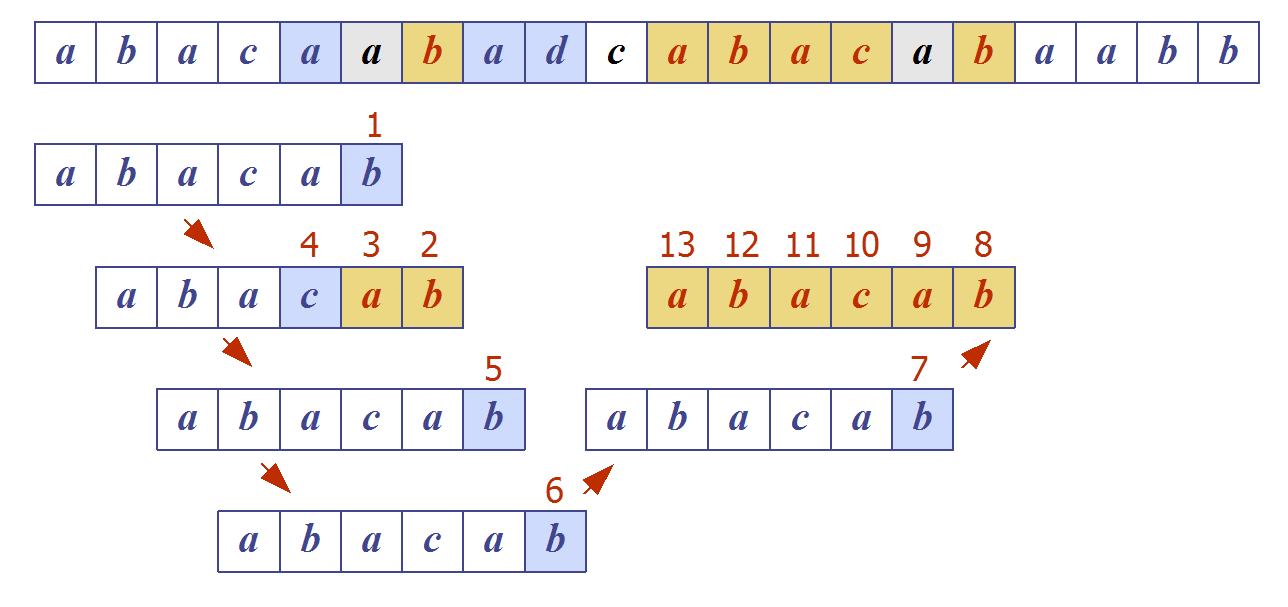
\includegraphics[width=11cm]{asp-13-pic03.png}
  \end{center}
\end{frame}

\begin{frame}[fragile]
  \frametitle{Boyer-Moore: analiza}
  \begin{columns}
    \begin{column}[t]{6cm}
      \begin{itemize}
        \item Boyer-Moore je $O(nm+s)$
        \item primer najgoreg slučaja:
        \begin{itemize}
          \item $T = aaa \ldots a$
          \item $P = baaa$
        \end{itemize}
        \item najgori slučaj nije verovatan u tekstovima
        \item znatno brži od grube sile za tekstove na prirodnom jeziku
      \end{itemize}
    \end{column}
    \begin{column}[t]{6cm}
      \begin{center}
        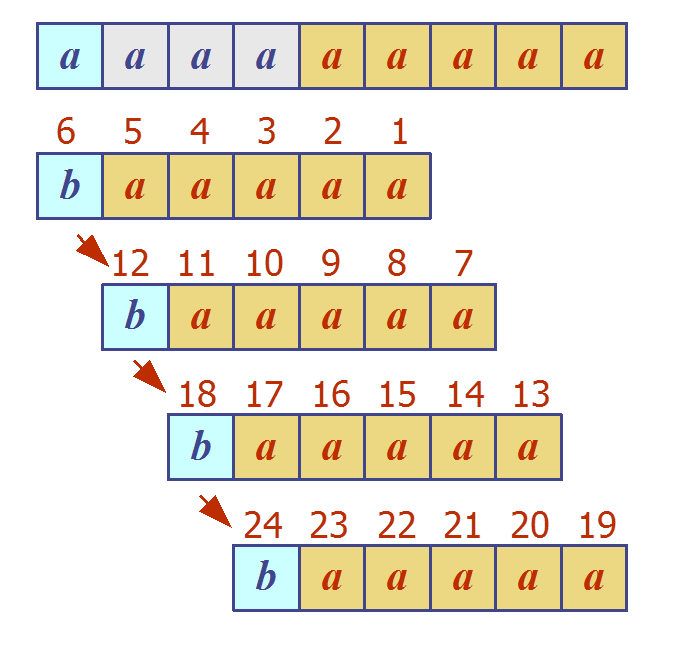
\includegraphics[width=6cm]{asp-13-pic04.png}
      \end{center}
    \end{column}
  \end{columns}
\end{frame}

\begin{frame}[fragile,shrink]
  \frametitle{Boyer-Moore u Pythonu}
\begin{minted}[linenos=false]{python}
def find_boyer_moore(T, P):
  """Return the lowest index of T at which substring P begins (or else -1)."""
  n, m = len(T), len(P)                   # introduce convenient notations
  if m == 0: return 0                     # trivial search for empty string
  last = {}                               # build 'last' dictionary
  for k in range(m):
    last[ P[k] ] = k                      # later occurrence overwrites
  # align end of pattern at index m-1 of text
  i = m-1                                 # an index into T
  k = m-1                                 # an index into P
  while i < n:
    if T[i] == P[k]:                      # a matching character
      if k == 0:
        return i                          # pattern begins at index i of text
      else:
        i -= 1                            # examine previous character
        k -= 1                            # of both T and P
    else:
      j = last.get(T[i], -1)              # last(T[i]) is -1 if not found
      i += m - min(k, j + 1)              # case analysis for jump step
      k = m - 1                           # restart at end of pattern
  return -1
\end{minted}
\end{frame}

\begin{frame}[fragile]
  \frametitle{Knuth-Morris-Pratt}
  \begin{columns}
    \begin{column}[t]{6cm}
      \begin{itemize}
        \item \myred{Knuth-Morris-Pratt} poredi tekst sa šablonom \textbf{sleva
        u desno} ali pomera šablon pametnije od grube sile
        \item kada se nađe razlika, koliko \textbf{najviše} možemo pomeriti
        šablon da izbegnemo suvišna poređenja?
        \item odgovor: najveći prefiks $P[0..j]$ koji je sufiks $P[1..j]$
      \end{itemize}
    \end{column}
    \begin{column}[t]{6cm}
      \begin{center}
        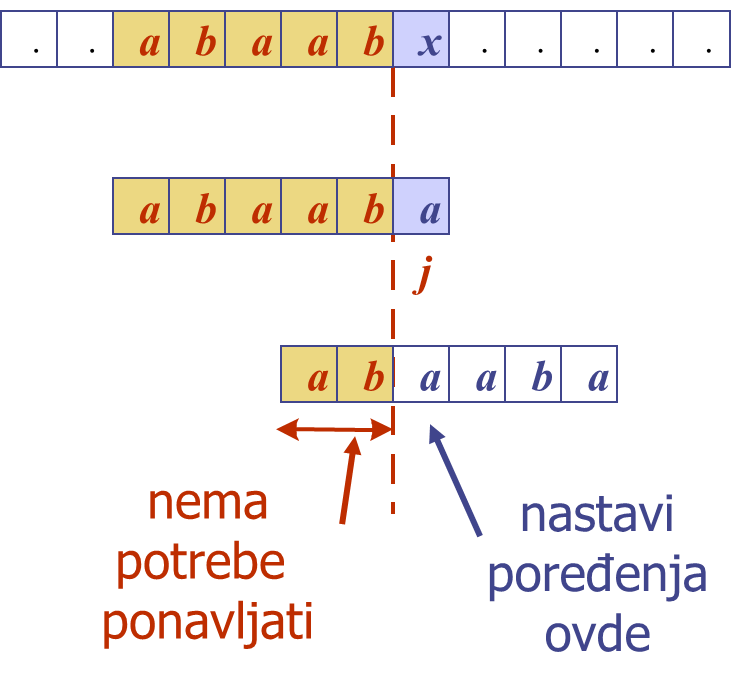
\includegraphics[width=6cm]{asp-13-pic05.png}
      \end{center}
    \end{column}
  \end{columns}
\end{frame}

\begin{frame}[fragile]
  \frametitle{KMP: funkcija neuspeha}
  \begin{columns}
    \begin{column}[t]{6cm}
      \begin{itemize}
        \item KMP analizira šablon da pronađe njegove prefikse unutar samog
        šablona
        \item \myred{funkcija neuspeha} $F(j)$ je veličina najvećeg prefiksa
        $P[0..j]$ takvog da je ujedno i sufiks $P[1..j]$
        \item razlika KMP i GS: ako nema poklapanja za $P[j] \neq T[i]$ pomeramo
        $j \leftarrow F(j-1)$
      \end{itemize}
    \end{column}
    \begin{column}[t]{6cm}
      \begin{center}
        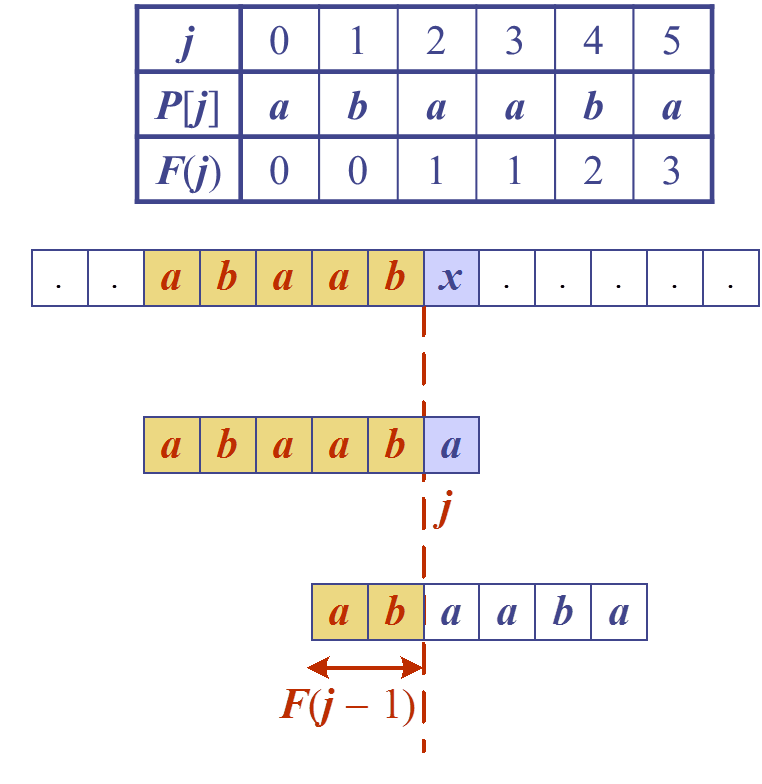
\includegraphics[width=6cm]{asp-13-pic06.png}
      \end{center}
    \end{column}
  \end{columns}
\end{frame}

\begin{frame}[fragile,shrink=12]
  \frametitle{Knuth-Morris-Pratt algoritam}
  \begin{columns}
    \begin{column}[t]{6cm}
      \begin{itemize}
        \item funkcija neuspeha se može prikazati nizom koji se izračuna za $O(m)$
        \item u svakoj iteraciji petlje, ili
        \begin{itemize}
          \item $i$ se poveća za $1$, ili
          \item pomeraj $i-j$ se poveća za najmanje $1$ (primeti da $F(j-1)<j$)
        \end{itemize}
        \item $\Rightarrow$ nema više od $2n$ iteracija u petlji
        \item $\Rightarrow$ KMP je $O(m+n)$
      \end{itemize}
    \end{column}
    \begin{column}[t]{6cm}
      \myred{KMPMatch}($T, P$)
      \begin{algorithmic}
        \STATE $F \leftarrow$ failureFunction($P$)
        \STATE $i \leftarrow 0$
        \STATE $j \leftarrow 0$
        \WHILE{$i<n$}
          \IF{$T[i]=P[j]$}
            \IF{$j=m-1$}
              \RETURN $i-j$ \COMMENT{poklapanje}
            \ELSE
              \STATE $i \leftarrow i+1$
              \STATE $j \leftarrow j+1$
            \ENDIF
          \ELSE
            \IF{}
              \STATE $j \leftarrow F[j-1]$
            \ELSE
              \STATE $i \leftarrow i + 1$
            \ENDIF
          \ENDIF
        \ENDWHILE
        \RETURN $-1$ \COMMENT{nije pronađen}
      \end{algorithmic}    
    \end{column}
  \end{columns}
\end{frame}

\begin{frame}[fragile,shrink=12]
  \frametitle{KMP: izračunavanje funkcije neuspeha}
  \begin{columns}
    \begin{column}[t]{6cm}
      \begin{itemize}
        \item funkcija neuspeha se može prikazati nizom koji se izračuna za $O(m)$
        \item slično kao i sam KMP algoritam
        \item u svakoj iteraciji petlje, ili
        \begin{itemize}
          \item $i$ se poveća za $1$, ili
          \item pomeraj $i-j$ se poveća za najmanje $1$ (primeti da $F(j-1)<j$)
        \end{itemize}
        \item $\Rightarrow$ nema više od $2n$ iteracija u petlji
      \end{itemize}
    \end{column}
    \begin{column}[t]{6cm}
      \myred{failureFunction}($P$)
      \begin{algorithmic}
        \STATE $F[0] \leftarrow 0$
        \STATE $i \leftarrow 1$
        \STATE $j \leftarrow 0$
        \WHILE{$i<m$}
          \IF{$P[i]=P[j]$}
            \STATE \COMMENT{poklapa se $j+1$ znakova}
            \STATE $F[i] \leftarrow j+1$
            \STATE $i \leftarrow i+1$
            \STATE $j \leftarrow j+1$
          \ELSIF{$j>0$}
            \STATE \COMMENT{koristi fF da pomeriš $P$}
            \STATE $j \leftarrow F[j-1]$
          \ELSE
            \STATE $F[0] \leftarrow 0$ \COMMENT{nema poklapanja}
            \STATE $i \leftarrow i + 1$
          \ENDIF
        \ENDWHILE
      \end{algorithmic}    
    \end{column}
  \end{columns}
\end{frame}

\begin{frame}[fragile]
  \frametitle{Knuth-Morris-Pratt: primer}
  \begin{center}
    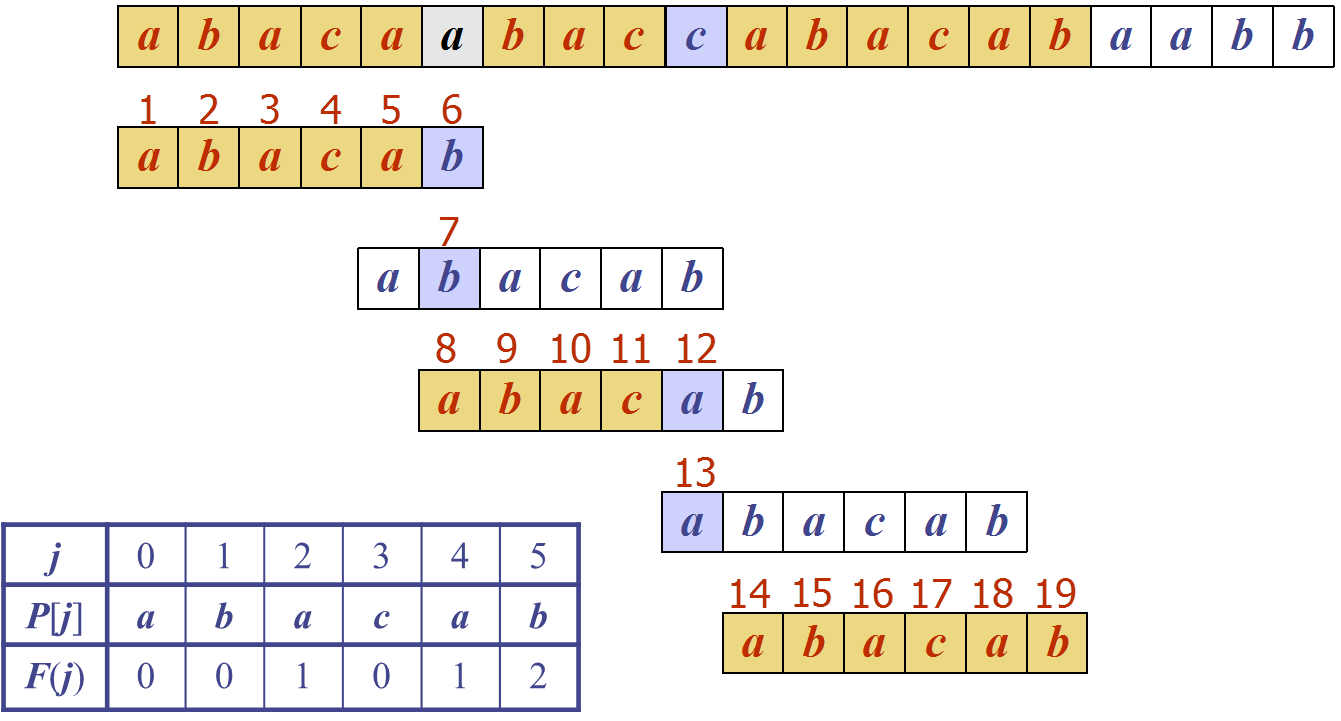
\includegraphics[width=11cm]{asp-13-pic07.png}
  \end{center}
\end{frame}

\begin{frame}[fragile,shrink]
  \frametitle{Knuth-Morris-Pratt u Pythonu $_1$}
\begin{minted}[linenos=false]{python}
def find_kmp(T, P):
  """Return the lowest index of T
     at which substring P begins (or else -1)."""
  n, m = len(T), len(P)       # introduce convenient notations
  if m == 0: return 0         # trivial search for empty string
  fail = compute_kmp_fail(P)  # rely on utility to precompute
  j = 0                       # index into text
  k = 0                       # index into pattern
  while j < n:
    if T[j] == P[k]:          # P[0:1+k] matched thus far
      if k == m - 1:          # match is complete
        return j - m + 1           
      j += 1                  # try to extend match
      k += 1
    elif k > 0:                    
      k = fail[k-1]           # reuse suffix of P[0:k]
    else:
      j += 1
  return -1                   # reached end without match
\end{minted}
\end{frame}

\begin{frame}[fragile,shrink=12]
  \frametitle{Knuth-Morris-Pratt u Pythonu $_2$}
\begin{minted}[linenos=false]{python}
def compute_kmp_fail(P):
  """Utility that computes and returns KMP 'fail' list."""
  m = len(P)
  fail = [0] * m    # by default, presume overlap of 0 everywhere
  j = 1
  k = 0
  while j < m:        # compute f(j) during this pass, if nonzero
    if P[j] == P[k]:  # k + 1 characters match thus far
      fail[j] = k + 1
      j += 1
      k += 1
    elif k > 0:       # k follows a matching prefix
      k = fail[k-1]
    else:             # no match found starting at j
      j += 1
  return fail
\end{minted}
\end{frame}

\section[Din prog]{Dinamičko programiranje}

\begin{frame}[fragile]
  \frametitle{Dinamičko programiranje}
  \begin{columns}
    \begin{column}[t]{6cm}
      \begin{itemize}
        \item \myred{dinamičko programiranje} je pristup dizajnu algoritama
        \item prvo primer: množenje matrica
        $$ C[i,j] = \sum_{k=0}^{e-1} A[i,k]\cdot B[k,j]$$
        \item vreme je $O(def)$
      \end{itemize}
    \end{column}
    \begin{column}[t]{6cm}
      \begin{center}
        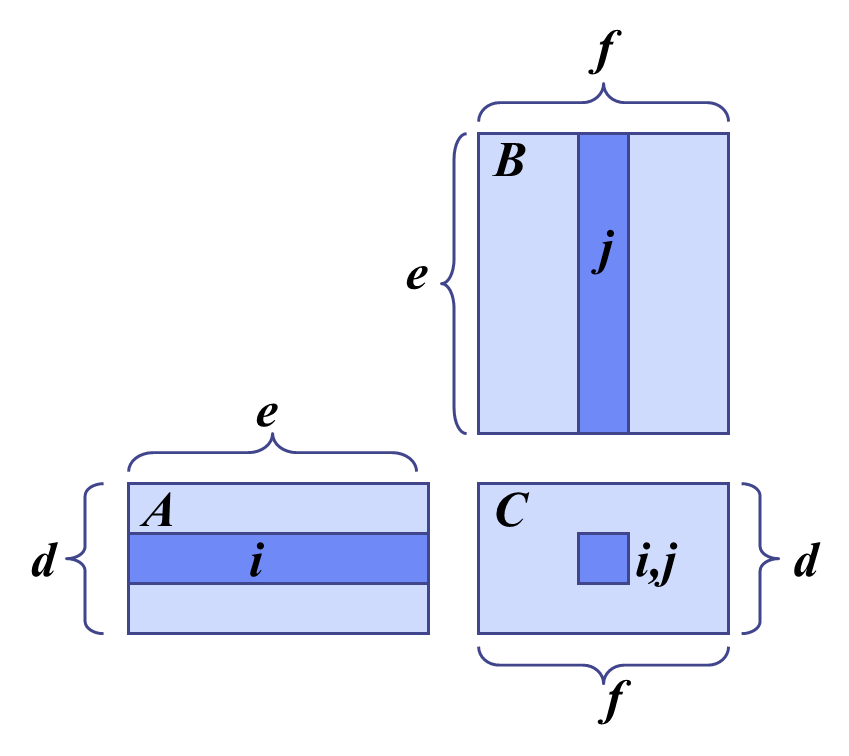
\includegraphics[width=6cm]{asp-13-pic08.png}
      \end{center}
    \end{column}
  \end{columns}
\end{frame}

\begin{frame}[fragile]
  \frametitle{Množenje matrica}
  \begin{itemize}
    \item računamo $A=A_0 \cdot A_{1}\cdot \ldots\cdot A_{n-1}$
    \item $A_{i}$ ima dimenzije $d_{i}\times d_{i+1}$
    \item koji redosled množenja izabrati?
    \item primer:
    \begin{itemize}
      \item $B$ je $3\times 100$
      \item $C$ je $100\times 5$
      \item $D$ je $5\times 5$
      \item $(B\cdot C)\cdot D$ traži 1500+75 = 1575 operacija
      \item $B\cdot (C\cdot D)$ traži 1500+2500 = 4000 operacija
    \end{itemize}
  \end{itemize}
\end{frame}

\begin{frame}[fragile]
  \frametitle{Raspoređivanje zagrada / gruba sila}
  \begin{itemize}
    \item traženje rešenja grubom silom: isprobati sve moguće 
    kombinacije zagrada za $A=A_0 \cdot A_{1}\cdot \ldots\cdot A_{n-1}$ 
    \item izračunati broj operacija za svaku
    \item i izabrati najbolju
    \item vreme izvršavanja:
    \begin{itemize}
      \item broj mogućih rasporeda zagrada je jednak broju različitih 
      binarnih stabala sa $n$ čvorova
      \item \textbf{eksponencijalna} zavisnost!
      \item tzv. Katalanov broj, iznosi skoro $4^n$
    \end{itemize}
  \end{itemize}
\end{frame}

\begin{frame}[fragile]
  \frametitle{Pohlepni pristup}
  \begin{itemize}
    \item ideja \#1: ponavljaj izbor onog proizvoda koji će imati \textbf{najviše} operacija
    \item protiv-primer:
    \begin{itemize}
      \item $A$ je $10\times 5$
      \item $B$ je $5\times 10$
      \item $A$ je $10\times 5$
      \item $B$ je $5\times 10$
      \item ideja \#1 daje $(A\cdot B)\cdot (C\cdot D)$, \\ tj. 500+1000+500 = 2000 operacija
      \item $A\cdot ((B\cdot C)\cdot D)$ je 500+250+250 = 1000 operacija
    \end{itemize}
  \end{itemize}
\end{frame}

\begin{frame}[fragile]
  \frametitle{Pohlepni pristup}
  \begin{itemize}
    \item ideja \#2: ponavljaj izbor onog proizvoda koji će imati \textbf{najmanje} operacija
    \item protiv-primer:
    \begin{itemize}
      \item $A$ je $101\times 11$
      \item $B$ je $11\times 9$
      \item $A$ je $9\times 100$
      \item $B$ je $100\times 99$
      \item ideja \#2 daje $A\cdot ((B\cdot C)\cdot D)$, \\ tj. 109989+9900+108900 = 228789 operacija
      \item $(A\cdot B)\cdot (C\cdot D)$ je 9999+89991+89100 = 189090 operacija
    \end{itemize}
    \item pohlepni pristup ne donosi optimalan izbor
  \end{itemize}
\end{frame}

\begin{frame}[fragile]
  \frametitle{,,Rekurzivni`` pristup}
  \begin{itemize}
    \item definišemo \myred{potprobleme}
    \begin{itemize}
      \item nađi najbolji raspored zagrada za $A_{i}\cdot A_{i+1}\cdot \ldots A_{j}$
      \item neka je $N_{i,j}$ broj operacija za ovaj potproblem
      \item optimalno rešenje za ceo problem je $N_{0,n-1}$
    \end{itemize}
    \item \myred{optimalnost potproblema}: optimalno rešenje se može 
    dobiti pomoću optimalnih potproblema
    \begin{itemize}
      \item mora postojati poslednje množenje (koren stabla izraza) za 
      optimalno rešenje
      \item neka je to na $i$-tom indeksu: $(A_{0}\cdot \ldots \cdot A_{i})\cdot (A_{i+1}\cdot \ldots \cdot A_{n-1})$
      \item optimalno rešenje za ceo problem $N_{0,n-1}$ je suma dva optimalna potproblema plus poslednje množenje
      \item ako bi optimalno rešenje imalo bolje potprobleme, ne bi bilo optimalno
    \end{itemize}
  \end{itemize}
\end{frame}

\begin{frame}[fragile]
  \frametitle{Karakteristična jednačina}
  \begin{itemize}
    \item globalni optimum se definiše pomoću optimalnih potproblema u 
    zavisnosti od indeksa poslednjeg množenja
    \item razmotrimo sve moguće vrednosti tog indeksa
    \begin{itemize}
      \item $A_{i}$ je dimenzije $d_{i}\times d_{i+1}$
      \item karakteristična jednačina za $N_{i,j}$ je:
      $$ N_{i,j} = \min_{i\leq k<j}\{ N_{i,k} + N_{k+1,j} + d_{i} d_{k+1} d_{j+1}\}$$
    \end{itemize}
    \item potproblemi nisu nezavisni, nego se \myred{preklapaju}
  \end{itemize}
\end{frame}

\begin{frame}[fragile]
  \frametitle{Algoritam dinamičkog programiranja}
  \begin{itemize}
    \item pošto se problemi preklapaju, nećemo koristiti rekurziju
    \item konstruisaćemo optimalne potprobleme od dole na gore (\textit{bottom-up})
    \item $N_{i,i}$ je lako, počnemo od njih
    \item onda pređemo na potprobleme dužine 2, 3, \ldots{}
    \item vreme izvršavanja je $O(n^3)$
  \end{itemize}
\end{frame}

\begin{frame}[fragile,shrink]
  \frametitle{Algoritam dinamičkog programiranja}
  \myred{matrixChain}($S$)
  \begin{algorithmic}
    \REQUIRE sekvenca $S$ matrica koje treba pomnožiti
    \ENSURE broj operacija u optimalnom rasporedu zagrada
    \FOR{$i \leftarrow 0$ \TO $n-1$}
      \STATE $N_{i,i} \leftarrow 0$
    \ENDFOR
    \FOR{$b \leftarrow 1$ \TO $n-1$}
      \FOR{$i \leftarrow 0$ \TO $n-b-1$}
        \STATE $j \leftarrow i+b$
        \STATE $N_{i,j} \leftarrow +\infty$
        \FOR{$k \leftarrow j-1$ \TO $j-1$}
          \STATE $N_{i,j} \leftarrow \min_{k} \{ N_{i,k} + N_{k+1,j} + d_{i} d_{k+1} d_{j+1}\}$
        \ENDFOR
      \ENDFOR
    \ENDFOR
  \end{algorithmic}    
\end{frame}

\begin{frame}[fragile,shrink=15]
  \frametitle{Python implementacija}
\begin{minted}[linenos=false]{python}
def matrix_chain(d):
  """Return solution to the matrix chain problem.

  d is a list of n+1 numbers describing the dimensions of a chain of
  n matrices such that kth matrix has dimensions d[k]-by-d[k+1].
 
  Return an n-by-n table such that N[i][j] represents the minimum 
  number of multiplications needed to compute the product of Ai 
  through Aj inclusive.
  """
  n = len(d) - 1                  # number of matrices
  N = [[0] * n for i in range(n)] # initialize n-by-n result to zero
  for b in range(1, n):           # number of products in subchain
    for i in range(n-b):          # start of subchain
      j = i + b                   # end of subchain
      N[i][j] = min(N[i][k] + N[k+1][j] + d[i]*d[k+1]*d[j+1] \
        for k in range(i,j))
  return N
\end{minted}
\end{frame}

\begin{frame}[fragile,shrink]
  \frametitle{Vizuelizacija algoritma}
  \begin{columns}
    \begin{column}[t]{6cm}
      \begin{itemize}
        \item bottom-up prvo popuni dijagonalu
        \item $N_{i,j}$ se dobija na osnovu vrednosti iz $i$-tog reda i 
        $j$-te kolone
        \item popunjavanje svake ćelije u tabeli je $O(n)$
        \item ukupno vreme je $O(n^3)$
        \item raspored zagrada dobijamo pamćenjem $k$ u ćelijama tabele
      \end{itemize}
    \end{column}
    \begin{column}[t]{6cm}
      \begin{center}
        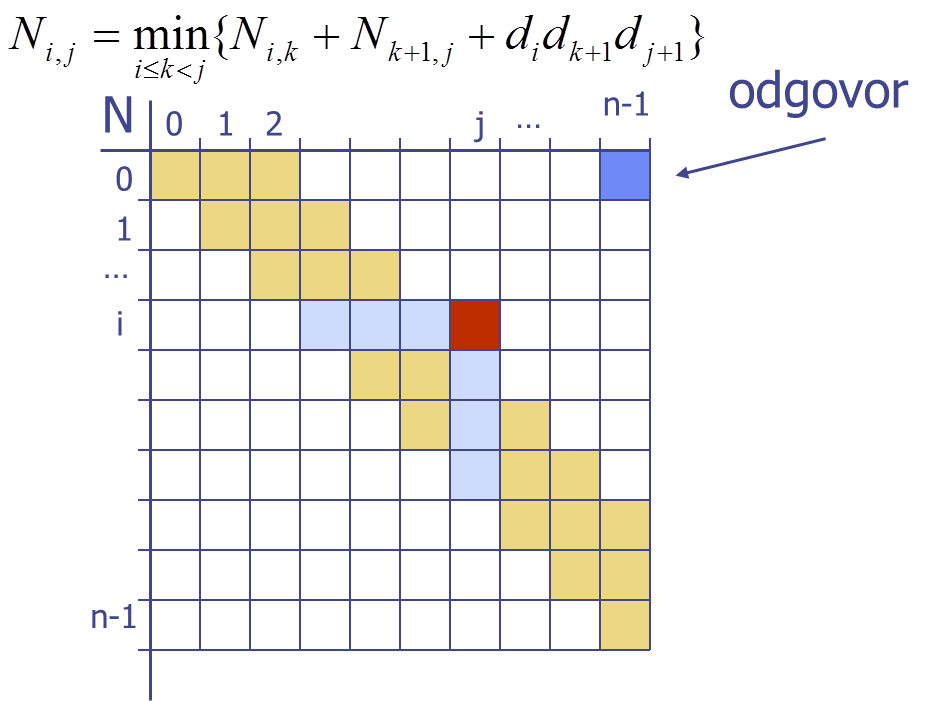
\includegraphics[width=6cm]{asp-13-pic09.png}
      \end{center}
    \end{column}
  \end{columns}
\end{frame}

\begin{frame}[fragile]
  \frametitle{Opšti postupak dinamičkog programiranja}
  \begin{itemize}
    \item primenljivo na probleme čije rešavanje traži puno vremena 
    (moguće eksponencijalni) ukoliko postoje:
    \begin{itemize}
      \item \myred{jednostavni potproblemi}: potproblemi se mogu 
      definisati pomoću promenljivih $j,k,l,m$ itd.
      \item \myred{optimalni potproblemi}: globalni optimum se može 
      definisati pomoću optimalnih potproblema
      \item \myred{preklapanje potproblema}: potproblemi nisu nezavisni
      i treba ih konstruisati bottom-up
    \end{itemize}
  \end{itemize}
\end{frame}

\begin{frame}[fragile]
  \frametitle{Podsekvence}
  \begin{itemize}
    \item \myred{podsekvenca} stringa $x_{0}x_{1}x_{2}\ldots x_{n-1}$ je
    string $x_{i_{1}}x_{i_{2}}\ldots x_{i_{k}}$ gde je $i_{j}<i_{j+1}$
    \item nije isto što i podstring!
    \item primer stringa: ABCDEFGHIJK
    \begin{itemize}
      \item jeste podsekvenca: ACEGIJK
      \item jeste podsekvenca: DFGHK
      \item nije podsekvenca: DAGH
    \end{itemize}
  \end{itemize}
\end{frame}

\begin{frame}[fragile]
  \frametitle{Problem najduže zajedničke podsekvence}
  \begin{itemize}
    \item \myred{longest common subsequence} (LCS)
    \item za stringove $X$ i $Y$, LCS je najduža podsekvenca od $X$ i $Y$
    \item primena: ispitivanje sličnosti DNK (alfabet je \{A,C,G,T\})
    \item primer: ABCDEFG i XZACKDFWGH imaju LCS: ACDFG
  \end{itemize}
\end{frame}

\begin{frame}[fragile]
  \frametitle{LCS grubom silom}
  \begin{itemize}
    \item primena grube sile na LCS:
    \begin{itemize}
      \item pronađi sve podsekvence od $X$
      \item izdvoj one koje su i podsekvence od $Y$
      \item izaberi najdužu
    \end{itemize}
    \item analiza:
    \begin{itemize}
      \item ako je $X$ dužine $n$, ima $2^n$ podsekvenci
      \item ovo je eksponencijalno vreme!
    \end{itemize}
  \end{itemize}
\end{frame}

\begin{frame}[fragile]
  \frametitle{LCS dinamičkim programiranjem}
  \begin{itemize}
    \item neka je $L[i,j]$ LCS za $X[0..i]$ i $Y[0..j]$
    \item neka postoji indeks -1, tako da je $L[-1,k]=0$ i $L[k,-1]=0$; 
    to znači da null deo X ili Y nema poklapanja sa drugim
    \item sada definišemo $L[i,j]$ u opštem slučaju:
    \begin{itemize}
      \item ako je $x_{i}=y_{j}$ onda $L[i,j] = L[i-1,j-1]+1$ \\ (imamo poklapanje)
      \item ako je $x_{i}\neq y_{j}$ onda $L[i,j] = \max\{L[i-1,j], L[i,j-1]\}$ \\ (nemamo poklapanje)
    \end{itemize}
  \end{itemize}
  \begin{center}
    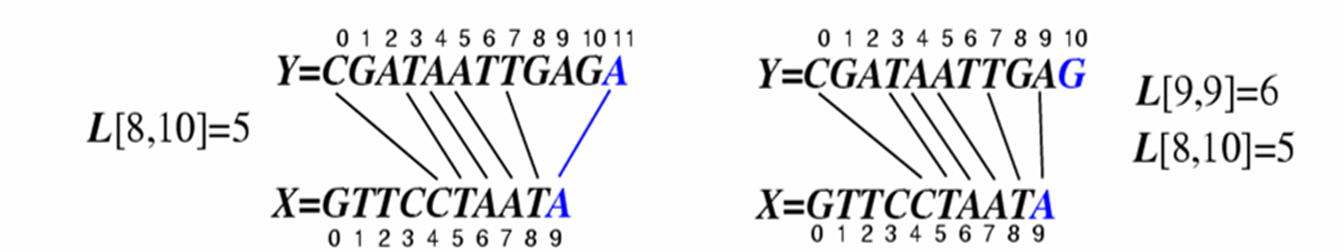
\includegraphics[width=11cm]{asp-13-pic10.png}
  \end{center}
\end{frame}

\begin{frame}[fragile,shrink]
  \frametitle{LCS algoritam}
  \myred{LCS}($X,Y$)
  \begin{algorithmic}
    \REQUIRE stringovi $X$ i $Y$ dužine $n$ odnosno $m$
    \ENSURE $L[i,j]$ za $0\leq i<n$ i $0\leq j<m$
    \FOR{$i \leftarrow 0$ \TO $n-1$}
      \STATE $N_{i,-1} \leftarrow 0$
    \ENDFOR
    \FOR{$j \leftarrow 0$ \TO $m-1$}
      \STATE $N_{-1,j} \leftarrow 0$
    \ENDFOR
    \FOR{$i \leftarrow 0$ \TO $n-1$}
      \FOR{$j \leftarrow 0$ \TO $m-1$}
        \IF{$x_{i} = y_{j}$}
          \STATE $L[i,j] \leftarrow L[i-1,j-1]+1$
        \ELSE
          \STATE $L[i,j] \leftarrow \max\{L[i-1,j], L[i,j-1]\}$
        \ENDIF
      \ENDFOR
    \ENDFOR
    \RETURN $L$
  \end{algorithmic}    
\end{frame}

\end{document}
